\appendix
\section{Nexys4 DDR开发板基本信息}

\begin{figure}[htbp]
    \centering
    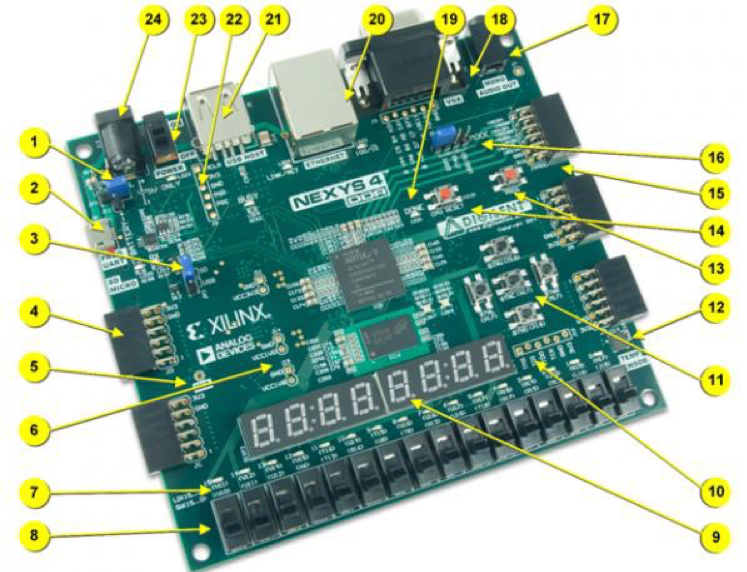
\includegraphics[width = 0.75\textwidth]{image/appendix/appendix_a_0.png}
    \caption{Nexys4 DDR示意图}
    \label{fig:appendix_a_0}
\end{figure}

\begin{table}[htbp]
    \centering
    \begin{tabular}{cc|cc}
         1& 选择供电跳线 &   13 & FPGA配置复位按键 \\
         2& UART/ JTAG 共用 USB 接口 &   14 & CPU 复位按键 (用于软核)\\
         3& 外部配置跳线柱(SD / USB) &   15& 模拟信号 Pmod 端口(XADC)\\
         4& Pmod 端口 &   16&编程模式跳线柱 \\
         5& 扩音器 &   17&音频连接口 \\
         6& 电源测试点 &   18& VGA 连接口\\
         7& 16 个 LED &   19& FPGA 编程完成 LED\\
         8& 16 个拨键开关&   20&以太网连接口 \\
         9& 8 位 7 段数码管&   21&USB 连接口 \\
         10& 可选用于外部接线的 JTAG 端口&  22&(工业用) PIC24 编程端口 \\
         11& 5 个按键开关 &  23& 电源开关\\
         12& 板载温度传感器 &  24&电源接口 \\
        %  & & & \\
    \end{tabular}
    \caption{Nexys4 DDR 功能表}
    \label{tab:my_label}
\end{table}

\newpage
\section{Nexys4 DDR引脚说明}
\textbf{100MHz时钟  E3}

按键、拨码管、LED、七段数码管、Reset:
\begin{figure}[htbp]
    \centering
    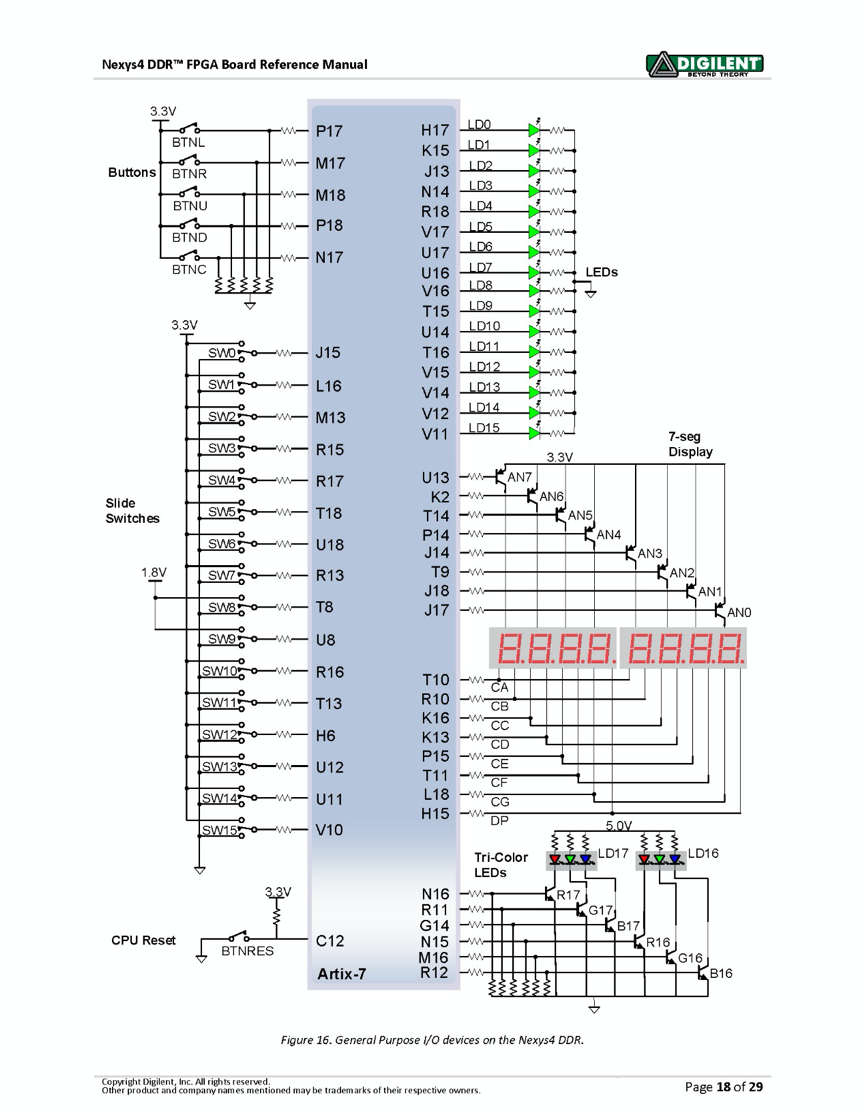
\includegraphics[width  = 0.9\textwidth]{image/appendix/appendix_b_0.png}
    \caption{Nexys4 DDR 管脚图}
    \label{fig:my_label}
\end{figure}

\newpage
\section{七段数码管的使用}
Nexys4 DDR实验板上有两个4位带小数点的七段数码管,图~\ref{fig:appendix_c_0}显示了它们与主芯片的连接方式。其中A7~A0是数码管8个位的使能信号,而CA~CG/DP则对应各个位上七个段以及小数点的触发信号。需要注意的是,使能信号和触发信号都是低电平触发的。

\begin{figure}[htbp]
    \centering
    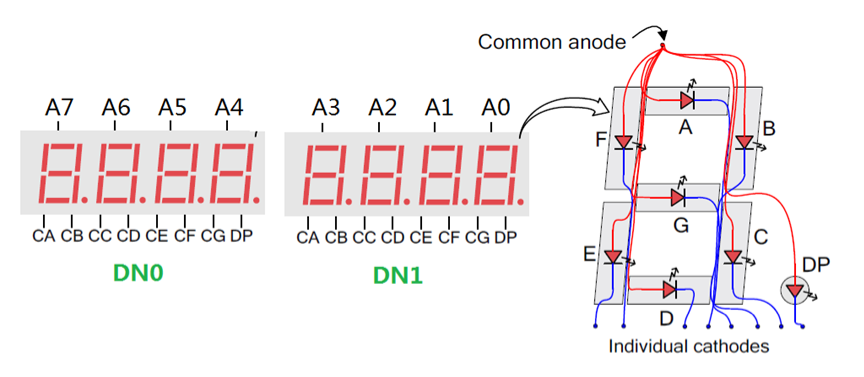
\includegraphics[width = \textwidth]{image/appendix/appendix_c_0.png}
    \caption{七段数码管示意图}
    \label{fig:appendix_c_0}
\end{figure}

图~\ref{fig:appendix_c_0}以数码管中最右侧的A0数码管为例说明了Nexys4 DDR板卡上的7-段数码管的连接方式。8个位中的各个相应的段及小数点分别连接到一组低电平触发的引脚上,他们被称为CA、CB、CC、…、CG、DP,其中,CA接到这8个数码管中每一个数码管A段的负极,CB接到这8个数码管中每一个数码管B段的负极,以此类推。

此外,每一个数码管都有一个使能信号A[7:0]。A[7:0]通过一个反相器接到对应数码管的每一个段的正极上。比如说,只有到A[0]为0的时候,最右侧数码管的显示才会受到CA…CG这几个信号的驱动。

图~\ref{fig:appendix_c_1}中列出了数码管显示0到F时点亮的段。比如说在显示数字0的时候,除了中间的G段外其他的段都被点亮了。而数字1只点亮了B段和C段。

\begin{figure}[htbp]
    \centering
    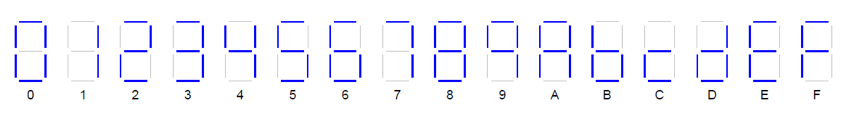
\includegraphics[width = \textwidth]{image/appendix/appendix_c_1.png}
    \caption{0-F点亮示意图}
    \label{fig:appendix_c_1}
\end{figure}

要想让每个数码管显示不同的数字,使能信号(A[7:0])和段信号(CA…CG)必须依次地被持续驱动,数码管之间的刷新速度应该足够快这样就看不出来数码管之间在闪烁。举个例子,如果想在数码管0上显示数字3而数码管1上显示数字9,可以先把CA…CG设置为显示数字3,并拉低A[1]信号,然后再把CA…CG设置为显示数字9并拉高A[1]拉低A[2]。刷新频率可以设置为2ms刷新一次,这样人眼就看不出闪烁了。